\chapter{Drawing Tools}\label{chap:chap2}
\special{pdf: out 1 << /Title (\thechapter. Drawing Tools) /Dest [ @thispage /FitH @ypos ] >>}

Placing the primitives mentioned in the chapter~\ref{chap:chap1} is usually not
sufficient to make a meaningfull drawing. So let's discuss other tools avialbale
in SteamCAD2.

\section{Selection}
\special{pdf: out 2 << /Title (\thesection. Selection) /Dest [ @thispage /FitH @ypos ] >>}

Once you finish drawing a primitive, you can escape the drawing mode pressing the ``Esc''
key and you get into selection mode. The selection mode operates in four ways:
\begin{enumerate}
\item Simple selection using mouse click. In this case all selected objects are unselected
and the newly clicked object is selected.
\item Multiple selection when holding down the Ctrl key. In this case the clicked
object is added to the selected set if it was previsously not selected. Otherwise
the object is deselected.
\item Multiple selection with dragging the left mouse button. In this case all the
objects fully covered by selection rectangle are selected.
\item Multiple selection with dragging the right mouse button. In this case only the
objects partially covered by selection rectangle are selected.
\end{enumerate}

You can combine the dragging rectangle selection with the Ctrl key to add objects
to the current selection set.

\section{Copying Objects}\label{sec:copyobj}
\special{pdf: out 2 << /Title (\thesection. Copying Objects) /Dest [ @thispage /FitH @ypos ] >>}

SteamCAD2 provides several methods to copy objects, including the clipboard. There
are four basic methods which simultaneously copy the object(s) and manipulate the copy:
\begin{enumerate}
\item \textbf{Copy Parallel}\label{sec:copypar} - this command is available with the shortcat
``Ctrl + C''. The selected object is coppied and placed upon left mouse click at a given
distance from the original object. The command works for all the primitive types, so it
actually creates a geometry equidistant from the original geometry. So for example an ellipse
coppied as ``parallel'' creates a curve which is not an ellipse anymore, except when
the distance from the original ellipse is zero. You can also copy parallel already copied
objects.

There is also an edit box in the status bar, where the exact distance can be specified.
If it contains valid number, the distance is locked and the mouse only controls on which
side from the origin the new object should be copied. Moreover, this only holds for
unbound curves. For bound or closed shapes, positive values copy the object to `ouside'
while negative values copy the object to `inside'. If the edit box is cleared or it
contains invalid distance value, the mouse controls both the position and the distance.
If the edit box already contains a value from previous commands, you can reuse this value
pressing the Enter key.

Also for Ellipse, Arc Ellipse, Hyperbola and Parabola, it is possible to move the copied
object further than is the smallest curve radius. In this case, while holding the Shift
key, you can move beyond the curve center. This is especially usefull for Ellipse and
Arc Ellipse.
\item \textbf{Move} - this command is available with the shortcut ``Alt + M''. Once activated,
two edit boxes appear in the status bar. You can enter the distance and the number of copies.
If you don't specify the number of copies, or set it to zero, no copy is created and
the object is simply moved. Otherwise the number of copies specified is created and
the objects are distributed uniformly along the move path.

If you specify the distance, you would be prompted to select a line to copy the
objects along. The positive direction is considered from left to right and from bottom
to top. You can also clear the distance edit box, in this case you will be prompted
to click two points - one for move ``from'' and the second for move ``to''.
\item \textbf{Rotate} - this command is available with the shortcut ``Ctrl + R''.
Similarly like with move command, you can provide the angle and number of copies.
If you don't specify the angle, you will be later prompted to click two points to
rotate ``from'' and to rotate ``to''. The command itself is activated by clicking
a point, which is the rotation origin.

If the angle to rotate is less than 360 degrees, the number of copies is the number
specified in the edit box. However, if the angle is equal to 360 degrees, the number
of copies is the number in the edit box minus 1. This is because the last copy
coincidents with the original. So for example, if you are designing a wheel with
10 spokes, you will draw 1 spoke and then rotate it by 360 degrees with 10 copies.
And the results will be exactly what you expect - 10 spokes ingluding the original one,
evenly distributed in the wheel rim.

This is for your convenience and it basically does the same, like rotating one spoke
for 360 - 36 degrees with 9 copies.
\item \textbf{Mirror} - this command is available with the shortcut ``Alt + I''.
This command is activated by clicking a line object to mirror the selected objects
around.
\item \textbf{Distribute} - this command is available with the shortcut ``Ctrl + D''.
It distributes selected objects along a curve or path. It has two variants.
If you put a positive number to the toolbar edit box, it create the requested number
of copies and distribute them along the clicked path. If ``keep orientation'' is
checked, then the objects are not rotated. Otherwise they are rotated by the curve
direction. Any object type including group and raster can be selected in this mode.

\begin{figure}[h]
\begin{center}
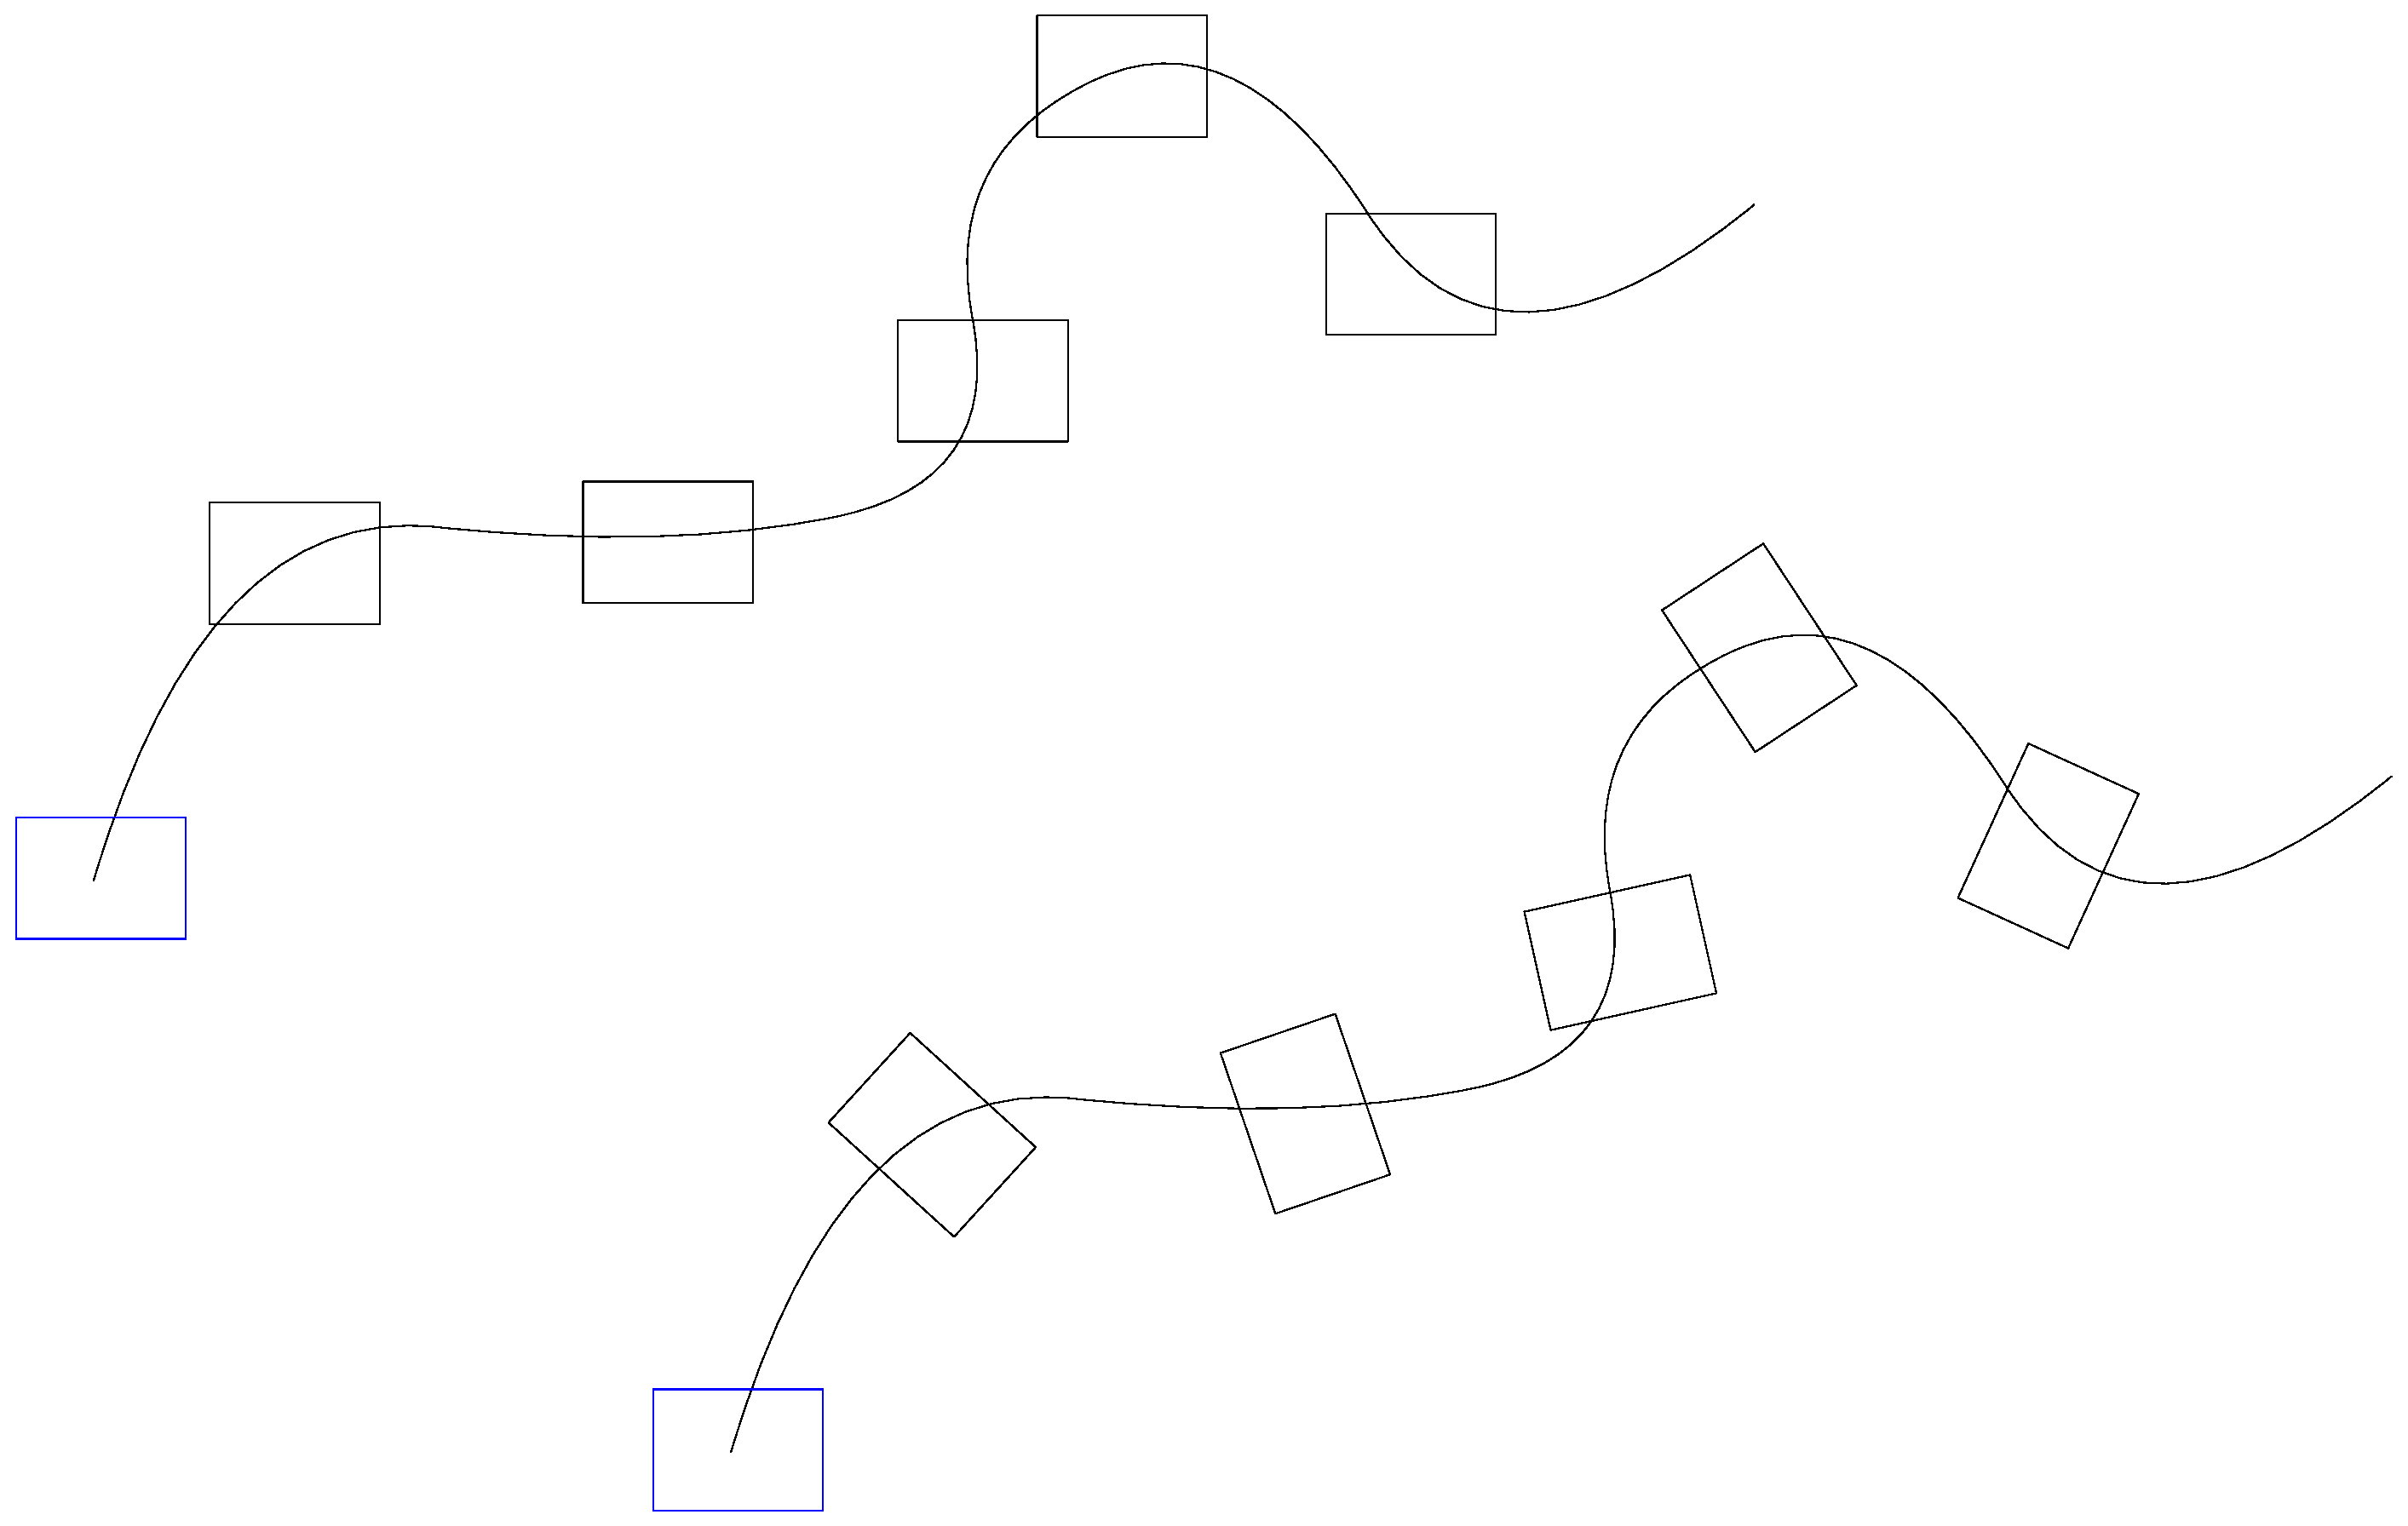
\includegraphics[scale=0.2]{Images/distr_fixed.eps}
\caption{Distribute in fixed mode with keeping orientation and without, the
original shape is blue}
\end{center}
\end{figure}

If the number of copies is zero or unspecified, then it attempts to distribute
the selected objects so that they are adjucent and fill the whole curve. We call
this \textbf{rubber mode}. The meaning should be clearer from the
figure~\ref{fig:distr_rubber}.
This mode has also two subvariants - when ``adjust to curvature'' is checked, then
the curve curvature (or radius) at given place is taken into account to make the
segments shorter or longer. Otherwise all the segments have the same length, so that
it fills the whole curve. This means that the shape can be slightly modified. The
selected objects to be distributed in rubber mode can only be linear segments or
paths consisting of linear segments only.

\begin{figure}[h]
\begin{center}
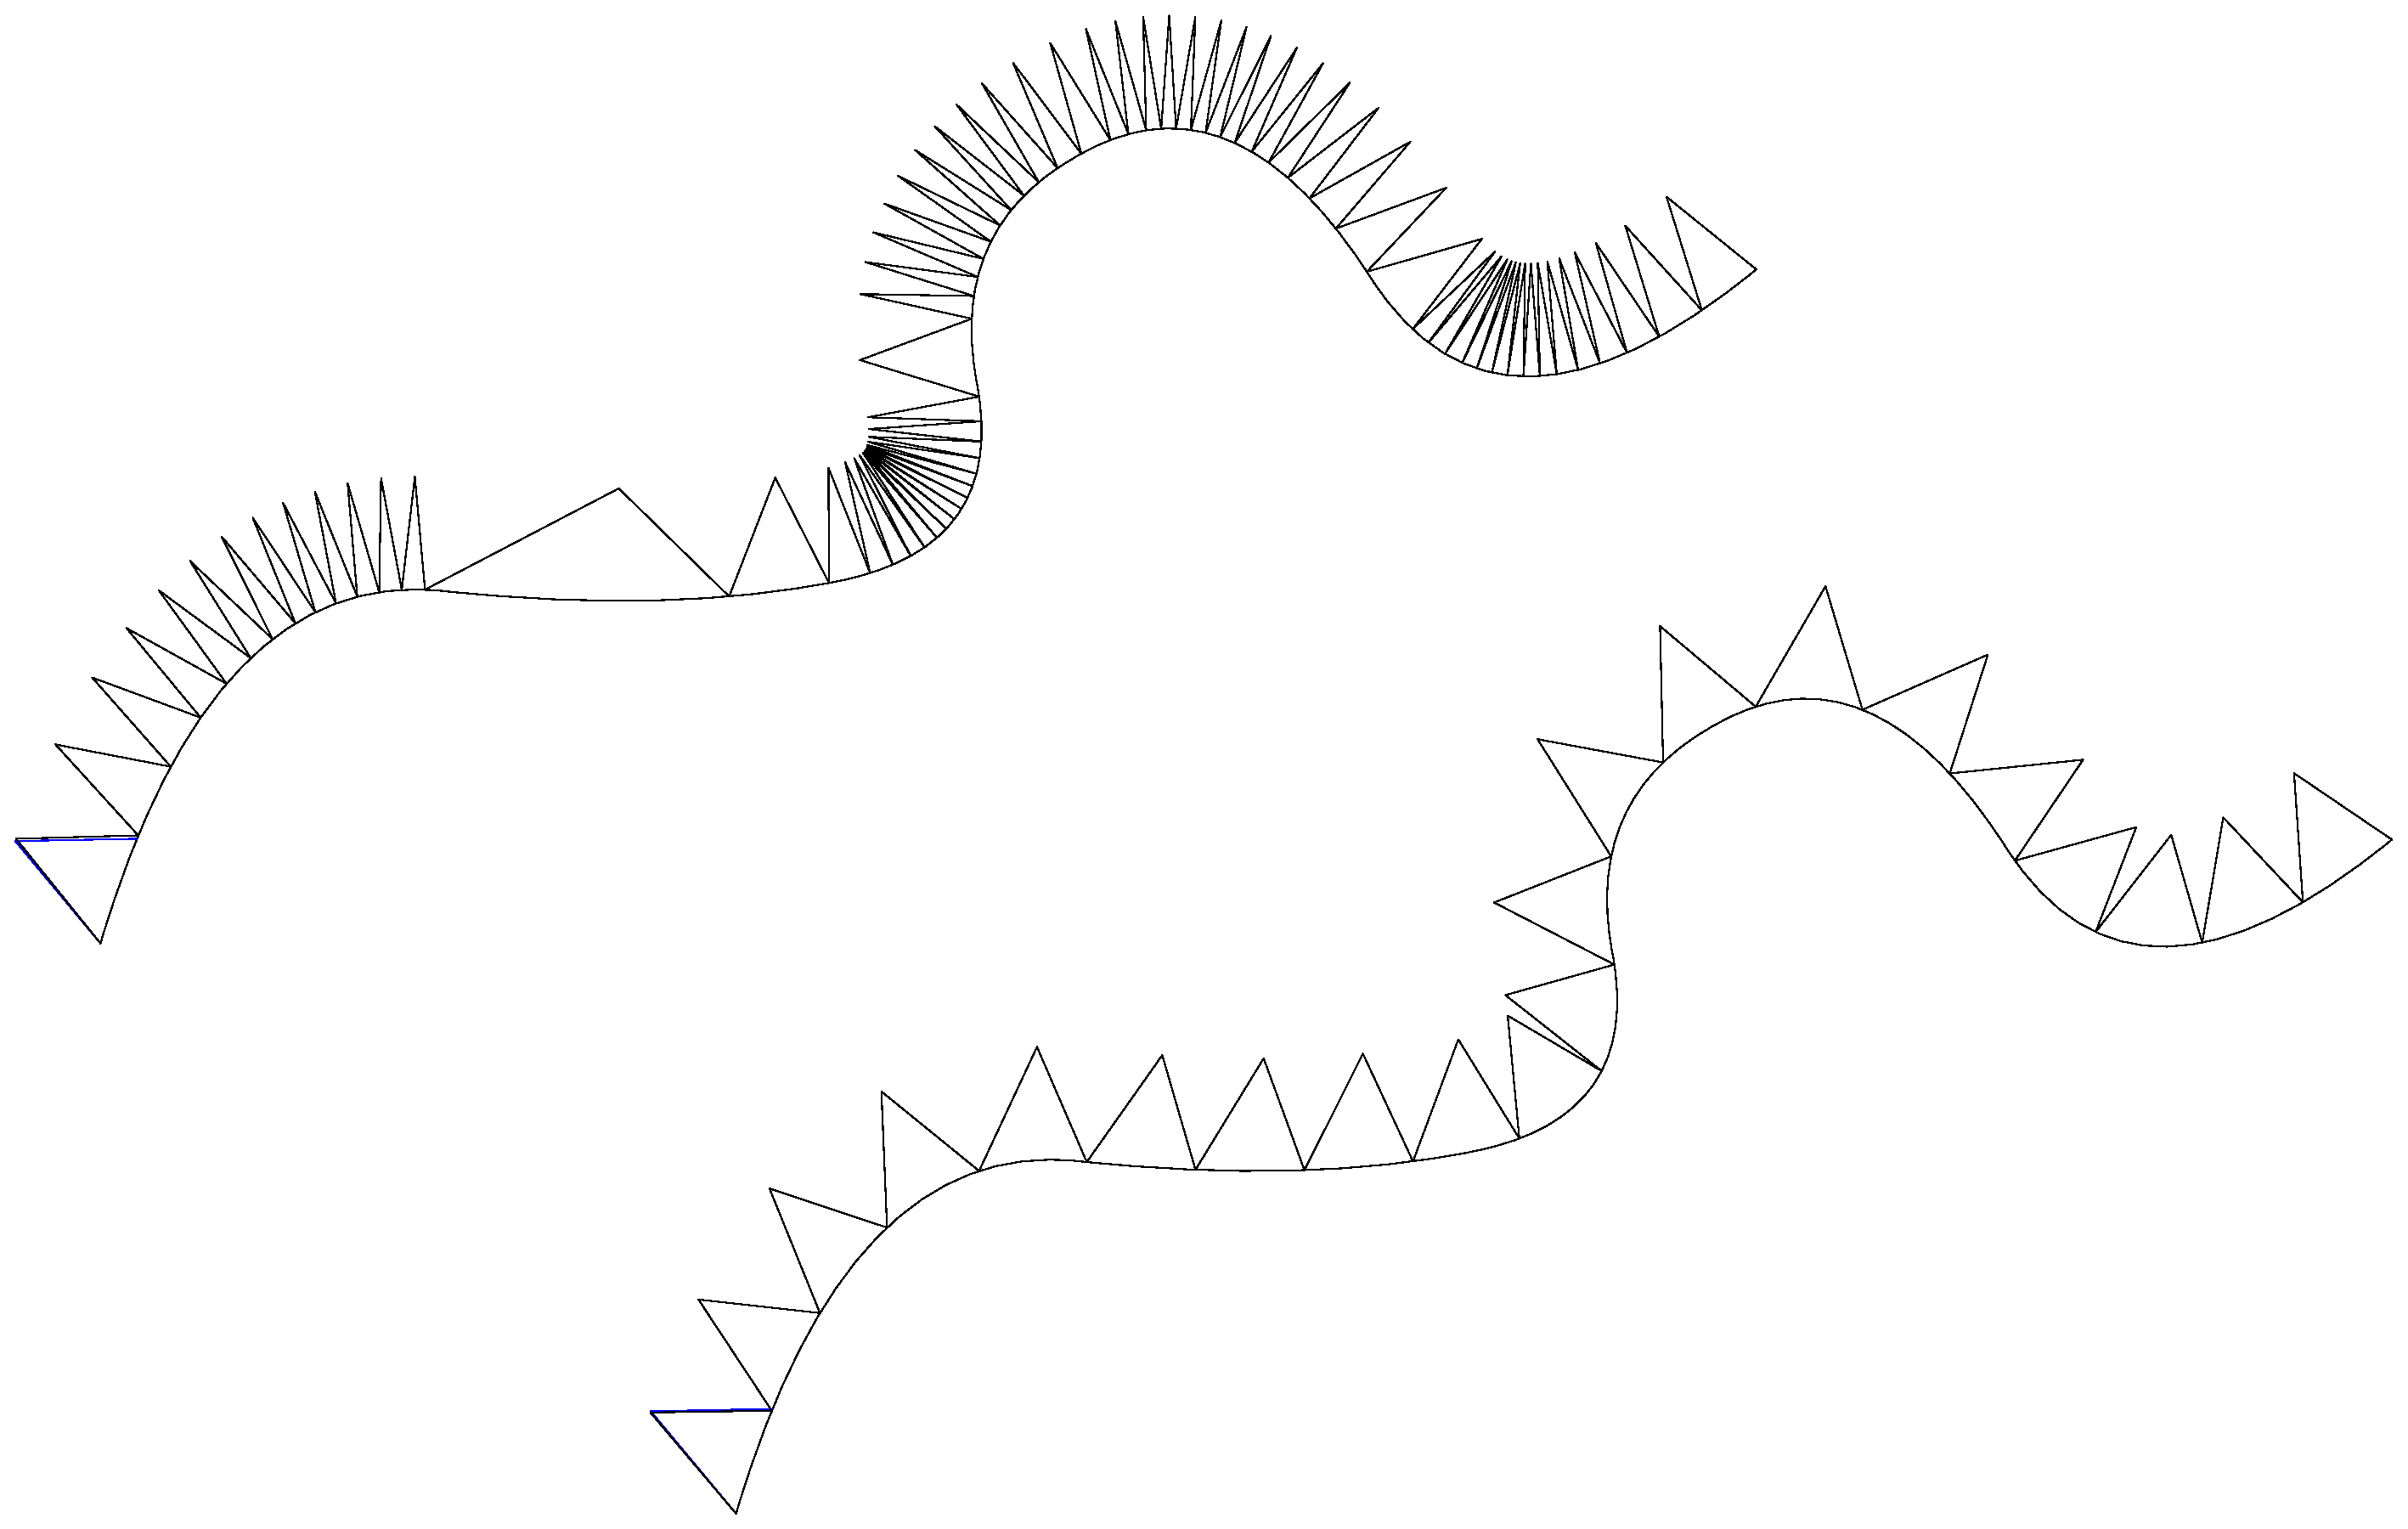
\includegraphics[scale=0.2]{Images/distr_rubber.eps}
\caption{Distribute in rubber mode with curvature adjustment and without, the
original shape is blue}
\label{fig:distr_rubber}
\end{center}
\end{figure}

\end{enumerate}

All the copy commands keep the original select set selected.

\section{Clipboard}
\special{pdf: out 2 << /Title (\thesection. Clipboard) /Dest [ @thispage /FitH @ypos ] >>}

SteamCAD2 provides standard clipboard both on Linux and Windows. Since from SteamCAD the
shortcut ``Ctrl + C'' is reserved for the copy parallel command, the standard Copy to
clipboard command is invoked by ``Alt + C''. The other two accompanying commands, Cut and
Paste, can be invoked by standard ``Ctrl + X'' and ``Ctrl + V'' shortcuts respectivelly.

\section{Deleting and Undoing Changes}
\special{pdf: out 2 << /Title (\thesection. Deleting and Undoing Changes) /Dest [ @thispage /FitH @ypos ] >>}

SteamCAD2 implements very little from usual Undo/Redo
commands. Here Undo and Redo only applies to deleted objects. You can delete the selected
objects simply by pressing the ``Delete'' key. All other SteamCAD2 operations can be
undone quite easily in a natural way, how we will see later.

A special case is when you are in the spline drawing mode. In this case, pressing the delete
key removes the last inserted point in the spline.

\section{Cutting and Extending Objects}\label{sec:extend}
\special{pdf: out 2 << /Title (\thesection. Cutting and Extending Objects) /Dest [ @thispage /FitH @ypos ] >>}

A line spanned accros all the paper is usually not what we would like to see in technical
drawings. So the next step is to trim the line to desired length. This is done by
activating the \textbf{Knife} command (``Alt + K'') and clicking the selected primitive at the
point you want to cut it. You can cut any number of selected primitives at once,
and you can also cut a single primitive as many times as you want. After you finish
with cutting, you can enter the selection mode and delete the unwanted parts.

A command complementary to Knife is called \textbf{Extend} (``Ctrl + E'') and it is
actually something like undo for knife. If you realize that a primitive is trimmed
at a wrong place, and the line is actually ``shorter'' than it should be, you can simply
activate the Extend command and click the end of the line, which should be extended.
The clicked half of the line is then restored to the original, unbounded shape.

SteamCAD2 moreover adds the abilitity to extend splines. If the spline is cut and the
user clicks on the cutted end, the spline is extended to its original state. However,
if the user clicks on the native start or end, the system gets into spline drawing mode
and new points can be added. This only holds for open splines, not for closed curves.

\section{Rounding Objects}
\special{pdf: out 2 << /Title (\thesection. Rounding Objects) /Dest [ @thispage /FitH @ypos ] >>}

The last command for creating shapes is called \textbf{Round} (``Ctrl + B'' - should have
been ``Bevel'' originaly, but later I realized that such a command can easily be replaced
by other tools). Selecting any two primitives, the command attempts to place a circular
arc tangent to both curves. You can also specify the radius of the arc. Unlike round
command in similar CAD system, the SteamCAD2's version does not modify the original
selected shapes. It's up to the user to trim them as appropriate.

\section{Edit spline}
\special{pdf: out 2 << /Title (\thesection. Edit spline) /Dest [ @thispage /FitH @ypos ] >>}

SteamCAD2 adds the ability to edit existing spline. Unlike other types of curves, spline
is a special case. It is often used for non-precise drawings thus having the possibility
to adjust the spline points may be useful. Using this command, the spline points can be moved,
added, selected and deleted by the ``Del'' key. It is also possible to extend spline using
the Extend command as described in~\ref{sec:extend}.

\section{Line Shaping}
\special{pdf: out 2 << /Title (\thesection. Line Shaping) /Dest [ @thispage /FitH @ypos ] >>}

Finally, when you finish drawing your shapes, you may want to specify the line
thickness and pattern. You can do this for the whole selected set at once, invoking
the \textbf{Line Style} dialog (``Alt + S''). Here you can specify the line width,
excentricity, translucency, blur (not implemented yet, maybe in the future), line
cap, line join, color and pattern.

The pattern should contain even number of values, every pair represents the length
of the line segment and the length of the hole. The odd numbers can also be zero,
in this case the pattern element is drawn as a point. Depending on the line cap,
it is either drawn like a circle or like a square. Don't use the zero length elements
with the line cap type ``Butt''. The zero elements might dissapear (on Linux).

The line excentricity means how much is the line set off its mathematical origin.
A typical usage of this parameter is whan drawing rails. Look at the introductory
image of the class 6 locomotive - the excentricity for rails is set to 100\%.
It means that the wheels and dimensions are properly aligned to the rails, while
the line is significantly thick to emphasize that this is actually the machine
base.

The line thickness can be an arbitrary decimal value. A positive value sets the
real line thickness in paper units. Lines with positive thickness are scaled
accordingly to the current zoom. A line with thickness zero is always drawn
as 1 pixel width, regardless the zoom. Lines with negative thicknes are drawn
scaled as positive lines, but only in SteamCAD2. Lines with negative
thicknes are not exported to the target format. Exports will be discussed later
in the section~\ref{sec:export}.


